\chapter[Solução]{Solução}

	\section[Solução Eletrônica]{Solução Eletrônica}
		\subsection[Sistema para controle de temperatura]{Sistema para controle de temperatura}
			O ideal para a manutenção das características do chopp é que o mesmo esteja armazenado na serpentina em uma temperatura de 0 $^{\circ}$C, e assim quando servido sua temperatura esteja entre 3 e 4$^{\circ}$ C e então sendo consumido entre 6 e 8 $^{\circ}$C. Afim de controlar a temperatura na serpentina será utilizado o sensor DS18B20, de acordo com a leitura fornecida o compressor será ativado ou não através de um relé e assim a temperatura será mantida dentro de uma margem previamente definida pelo sistema.

			\begin{figure}[H]
				\centering
				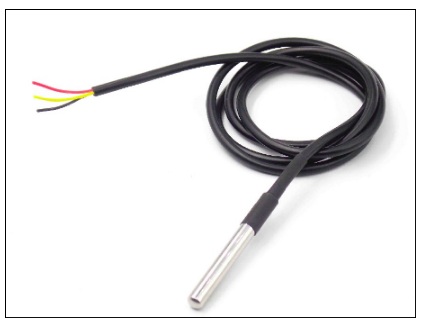
\includegraphics[scale= 0.7]{figuras/sensor-temperatura.png}
				\caption{Sensor DS18B20 utilizado para controle de temperatura.}
				\label{sensor-temperatura}
			\end{figure}

		\subsection[Sistema de tiragem de chopp]{Sistema de tiragem de chopp}
			\subsubsection[Estimar volume no copo]{Estimar volume no copo}
				A medição do volume presente no copo será dada de maneira empírica onde os testes com o sensor de 
				fluxo YFS201 , realizarão as medidas de fluxo e o controle de volume será dado através do tempo 
				estimado para a vazão de quantidades pré estabelecidas de chopp.

			\begin{figure}[H]
				\centering
				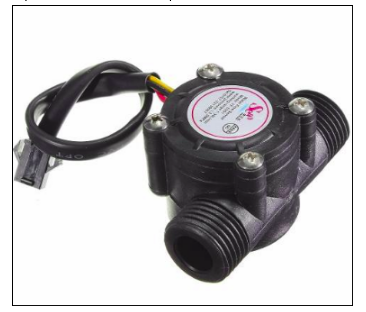
\includegraphics[scale= 0.7]{figuras/sensor-fluxo.png}
				\caption{Sensor de fluxo YFS201.}
				\label{sensor-fluxo}
			\end{figure}
			
			\subsubsection[Sistema de identificação de presença do copo]{Sistema de identificação de presença do copo}
				Afim de identificar a presença do copo no suporte da chopeira, será utilizado um sensor ultrasônico HC-SR04, que permite obter a distância entre o sensor e o primeiro obstáculo, no caso o copo. Com o dado dessa distância será identificado se o copo está no recinto ou não.

			\begin{figure}[H]
				\centering
				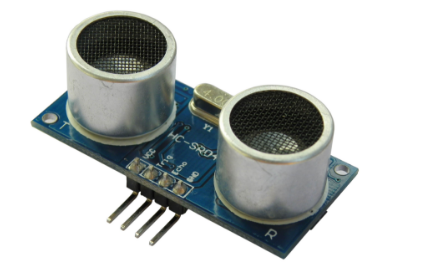
\includegraphics[scale= 0.7]{figuras/sensor-ultrassonico.png}
				\caption{Sensor ultrassônico HC-SR04.}
				\label{sensor-ultrassonico}
			\end{figure}

			\subsubsection[Sistema de inclinação do copo]{Sistema de inclinação do copo}
				Para que o chopp seja servido de forma adequada, a inclinação do copo é crucial no processo, para realizar essa inclinação um sistema mecânico será desenvolvido pela equipe de estrutura, já o acionamento desse mecanismo é promovido por um motor de passo bipolar, com capacidade de 200 passos por revolução, obtendo uma resolução de 1.8$^{\circ}$ por passo. Utilizando desse motor será feita a inclinação desejada.

			\begin{figure}[H]
				\centering
				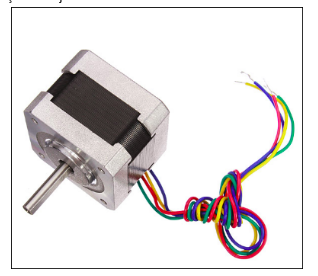
\includegraphics[scale= 0.7]{figuras/motor-passo.png}
				\caption{Motor de Passo Bipolar.}
				\label{motor-passo}
			\end{figure}
			
			\subsubsection[Estimar volume restante no barril]{Estimar volume restante no barril}
				Parte-se do princípio que aquele volume total presente no barril de chopp é conhecido inicialmente e toda variação representa necessariamente uma tiragem de chopp. Podem ser consideradas duas formas de se calcular o volume restante no barril de chopp. Elas são descritas a seguir e podem ser utilizadas de forma individual ou em conjunto, para dar redundância ao sistema. 

				O sensor de fluxo tem a capacidade de  medir o fluxo entre 1 e 30 litros  por minuto, com uma acurácia de 10 porcento e pode operar   numa faixa de temperatura entre -25 e 80 $^{\circ}$C.

				Para se calcular o volume restante no barril, sabendo o seu volume inicial, pode-se subtrair deste valor aquele do fluxo passando no sensor multiplicado pelo tempo de tiragem do chopp. Isso pode ser visto na Equação \ref{eq1}.

				\begin{equation} 
					\label{eq1}
					V_{restante} = V_{atual} -  {V_{passante}\over t}\times{t_{tiragem}}
				\end{equation}

				Por outro lado, uma célula de carga é um transdutor que  converte a pressão em sinais elétricos que podem ser medidos. Deste modo, medindo-se a massa massa inicial do barril e tendo seu volume inicial  conhecido, sua variação de volume pode ser calculada. A Figura \ref{celula-carga}  mostra um exemplo de célula de carga. 

				\begin{figure}[H]
					\centering
					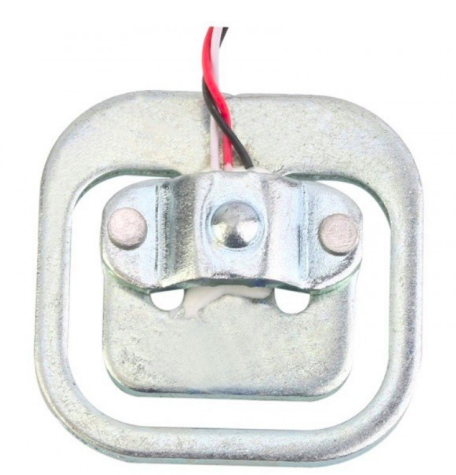
\includegraphics[scale= 0.7]{figuras/celula-carga.png}
					\caption{Exemplo de célula de carga.}
					\label{celula-carga}
				\end{figure}	

				Para que se calcule a variação de volume é preciso calcular a densidade inicial do sistema. A densidade é dada por uma quantidade de massa em uma quantidade de volume. Assim, posicionando-se os barris sobre células de carga pode-se medir a sua massa e tendo-se a massa de seus vasilhames conhecidas e fixa, tem-se a massa de líquido presente no sistema. 

				A partir do conhecimento da massa de líquido presente no sistema e tendo o volume total inicial conhecido, pode-se calcular o volume restante no sistema a partir da densidade. A Equação \ref{eq2} mostra como isso pode ser feito.
				 
				\begin{equation} 
					\label{eq2}
					V_{restante} = {M_{atual}\over D_{chopp}}
				\end{equation}				

			\subsubsection[Assegurar o tamanho do colarinho escolhido]{Assegurar o tamanho do colarinho escolhido}
				Para que se possa controlar o volume do colarinho do chopp, deve-se inicialmente controlar a 
				inclinação do copo durante a tiragem. Isso permite que se tenha o mínimo de colarinho durante o 
				período necessário para servir o chopp apenas e que se controle de forma mais precisa o colarinho.

		\subsection[Sistema de alimentação emergencial]{Sistema de alimentação emergencial}

			Para construção de um sistema inversor de DC para AC, será desenvolvido um circuito de ponte H com 
			transistores chaveados capaz de gerar uma tensão em senoidal que possa ser amplificada após a ponte a 
			partir de um transformador. A imagem \ref{circuito-inversor} indica o circuito simplificado proposto:

			\begin{figure}[H]
				\centering
				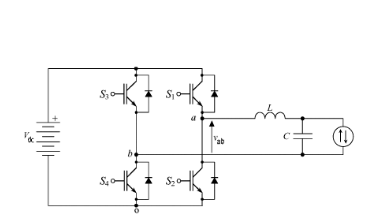
\includegraphics[scale= 0.7]{figuras/circuito-inversor.png}
				\caption{Exemplo de Circuito Inversor.}
				\label{circuito-inversor}
			\end{figure}

			As entradas S1, S2, S3, S4 serão chaveadas a partir de um microcontrolador AtTiny de forma que acione S1 
			junto com S3 ou S2 com S4 em uma frequência dentro de kHz de forma que na saída seja gerado uma onda 
			senoidal para alimentação do sistema.

			Para o circuito de retificação de AC para DC será utilizado um retificador simples para alimentar a 
			bateria do sistema de NoBreak. Esse circuito deve ser capaz de receber a tensão da rede (220 volts) e ter 
			a saída Para poder alimentar a bateria (12 volts). A imagem \ref{circuito-retificador} mostra o circuito simplificado do 
			retificador:

			\begin{figure}[H]
				\centering
				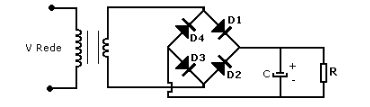
\includegraphics[scale= 0.7]{figuras/circuito-retificador.png}
				\caption{Exemplo de Circuito retificador.}
				\label{circuito-retificador}
			\end{figure}

	\section[Solução Software]{Solução Software}

		A solução de software foi dividida nos quatro subsistemas a seguir:

			\subsection[WebService]{WebService}
				A demanda do problema exige que diferentes hardwares se integrem com uma mesma base de dados. Fundamentalmente, o Smartphone do usuário realiza a compra, e o token deve reconhecer o ticket para que o usuário consuma o chopp.

				Para solucionar essa demanda é proposto uma arquitetura orientada a serviços (SOA), tal que uma webservice REST seja responsável pela persistência de todos os dados relevantes do sistema.
				
				A tecnologia escolhida para implementação desse sistema é o Ruby On Rails, pela facilidade no desenvolvimento, ampla comunidade e familiaridade e experiência da equipe.

			\subsection[Sistema mobile de compra]{Sistema mobile de compra}
				O subsistema mobile de compra será composto de um app que será utilizado por quem deseja comprar um chopp. Esse app se comunicará com o Webservice citado no tópico anterior.

				O comprador, ao utilizar o app, deve selecionar as preferências em relação ao chopp e após essa etapa, inserir os dados do cartão de crédito para efetuar o pagamento. Uma vez efetuado o pagamento, o sistema emitirá um código QR que deverá ser lido pela máquina para liberação do chopp.

				Para o desenvolvimento do app será utilizado o framework Ionic. Esse framework nos permite uma maior produtividade visto que podemos desenvolver um app multi-plataforma que atende tanto a plataforma Android quanto IOS. Dentre outras vantagens, o ionic também possui uma comunidade de desenvolvimento ampla comparada a outros frameworks multiplataformas como React Native.

			\subsection[Sistema Administrativo]{Sistema Administrativo}
				O subsistema mobile administrativo será composto de um aplicativo que será utilizado pelo responsável da máquina de chopp. Esse aplicativo possui uma comunicação direta com o sistema de Web Service anteriormente citado.

				O responsável pela máquina de chopp, deve fazer um cadastro no sistema onde os dados necessários para são o e-mail e a senha. Ao utilizar o aplicativo, o usuário visualizara as seguintes informações referentes ao estado da máquina: a quantidade de chopp que a máquina possui e o status da conexão da máquina com a internet e sistema de interação com o usuário. Quando algum desses parâmetros não estiver funcionando de maneira correta, o responsável pela máquina receberá uma notificação em seu smartphone para que providências sejam tomadas para correção desses problemas. 

				Esse sistema também será desenvolvido com uso da plataforma Ionic pelas mesmas vantagens que motivaram a escolha da plataforma no Sistema de Compra, até mesmo pela uniformidade das tecnologias, pensando nas evoluções dos sistemas.

			\subsection[Sistema de interação do usuário com a máquina]{Sistema de interação do usuário com a máquina}
				O sistema de interação do usuário com a chopeira vai permitir que após a compra do chopp pelo aplicativo mobile, o usuário interaja com a máquina e consiga pegar o chopp. Após a compra do chopp o usuário receberá um código QR (sigla do inglês para Quick Response - que é um código de barras bidimensional), que será mostrado à máquina para validação e início do preparo do chopp.
				
				A partir da interação inicial do usuário com a máquina, o sistema habilitará a câmera para a leitura do código QR. O usuário irá aproximar a tela do celular da câmera, que realizará a leitura. O sistema vai validar o código mostrado com o código armazenado no servidor, dará início ao processo de preparo do chopp e informará ao usuário quando o chopp estiver pronto.
				
				A solução será instalada na própria máquina, sobre o sistema operacional padrão da plataforma Raspberry, o Raspbian, com intuito de evitar incompatibilidade com outros sistemas operacionais e retrabalho. Além disso, com a intenção de manter o sistema alinhado à solução SOA, o sistema consumirá os serviços proporcionados pelo WebService. 


	\section[Solução Estrutura]{Solução Estrutura}

		\subsection[Estrutura]{Estrutura}
				Como citado anteriormente, um dos requisitos a serem atendidos pelo projeto estrutural é o de que as dimensões sejam adequadas para uma utilização confortável pelo usuário, que facilite manutenção e suporte de forma adequada e confiável todos os subsistemas da chopeira.
				
				Para isto, foram feitas análises prévias e estimativas dimensionais relacionadas a cada uma dessas necessidades. Podemos ver abaixo um esboço inicial da estrutura e as devidas considerações a respeito de alguns pontos chave do design.
				
				É importante frisar que o design final deve priorizar o alinhamento entre os requisitos funcionais e estéticos. Para que isso aconteça, o processo se torna altamente iterativo e envolve PDCA contínuo.

				\begin{figure}[H]
					\centering
					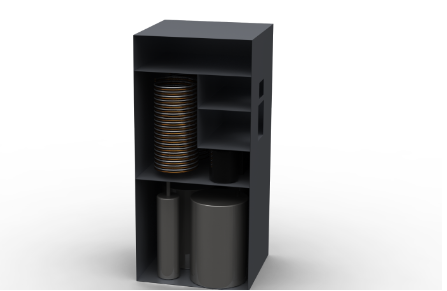
\includegraphics[scale= 0.7]{figuras/packaging-estrutura.png}
					\caption{Conceito inicial de packaging para a estrutura.}
					\label{packaging-estrutura}
				\end{figure}

				O primeiro objetivo funcional a ser definido para dimensionar a estrutura foi o packaging. Ele foi pensado de forma a alocar os subsistemas em níveis ao longo da estrutura. Partindo de baixo para cima, o primeiro nível seria dimensionado para alocar compressor e o sistema de alimentação de energia elétrica, bem como o sistema de emergência que entra em casos de falha na alimentação externa.
				
				O segundo nível seria destinado ao armazenamento dos barris de chopp e cilindros de CO2. Um dos pontos importantes desse nível é a facilidade de acesso e manutenção, pois provavelmente será o mais acessado ao longo do funcionamento, principalmente para fins de reposição. Diante dessa necessidade será instalada uma porta de manutenção de cada lado, de forma que cada barril (A capacidade será de 2 Barris de 50L) possa ser trocado sem que haja esforço físico elevado.
				
				O terceiro nível é onde se encontra toda a parte de refrigeração do chopp, este nível será forrado com manta térmica para melhor a eficiência do ciclo de refrigeração e o material empregado deve ser capaz de suportar temperaturas entre 0 e -10 graus Celsius sem perda significativa de resistência mecânica.
				
				Acima do terceiro nível da máquina existem mais dois compartimentos. O primeiro deles será destinado ao armazenamento de placas e circuitos eletrônicos bem como o Raspberry Pi, que será a base de todo sistema de gerenciamento da máquina.
				
				Esta localização para a parte eletrônica foi escolhida pois seria possível alocar os componentes diretamente atrás da tela do equipamento, o que reduziria a quantidade de fios, melhoraria o acabamento e reduziria pontos de possíveis falhas no sistema. A segurança no também tende a aumentar pois estando no ponto mais alto da máquina a chance de danos por umidade ou problemas relacionados ao sistema de refrigeração se reduz drasticamente.
				
				O último compartimento, localizado atrás dos circuitos eletrônicos será o de copos que a máquina disponibilizará para o usuário após pagamento. Neste nível o objetivo será ter um sistema simples e eficaz para a entrega dos copos. Isso será realizado pelo uso de um plano inclinado no interior do compartimento de uma porta controlada eletronicamente que será calibrada para liberar um copo a cada abertura. Esse copo cairá em uma bandeja e estará disponível para que o usuário possa pegá-lo.
				
				É importante frisar que a ergonomia foi pensada de forma que o usuário fizesse o mínimo de esforço possível para alcançar o seu objetivo, por esse motivo a tela de 7 polegadas será localizada de maneira a favorecer a utilização do público brasileiro (considerando homens e mulheres) e a entrada de copos será feita de forma que o braço consiga pegar sem que seja necessária extensão total do mesmo. 


		\subsection[Materiais e Resistência mecânica]{Materiais e Resistência mecânica}
			O principal objetivo no que tange ao projeto estrutural é obter máxima resistência mecânica aliada a baixo peso. Porém, materiais que permitem atingir esses dois objetivos mutuamente muitas vezes têm preços proibitivos.
			
			Os materiais mais apropriados e acessíveis para a fabricação da estrutura são alumínio e aço de baixo carbono, inclusive pela fácil disponibilidade.
			
			O aço possui excelente resistência mecânica na maioria de suas variações e com bom preço. No caso do alumínio, ligas de elevada resistência mecânica são caras, porém a capacidade de diminuir o peso final ao se utilizar esse material é considerável e bastante benéfica (O alumínio é cerca de 65\%\ menos denso do que o aço).

			Empregar alumínio em peças geometricamente fáceis de aplicar  e também em peças pouco solicitadas (Carcaça externa da máquina, bandeja de copos, suporte de componentes eletrônicos, portas de manutenção). Os componentes da estrutura que trabalham com solicitações mais severas e desfavoráveis serão fabricados em aço (suporte onde o Barril e o cilindro são apoiados, câmara de refrigeração, Alojamento do compressor e nobreak). Dessa forma teremos uma


	\section[Solução Energia]{Solução Energia}
		Nos diagramas a seguir podem ser verificados esboços do funcionamento geral do solução proposta e as macro entradas, saídas e riscos do projeto.

		\begin{figure}[H]
			\centering
			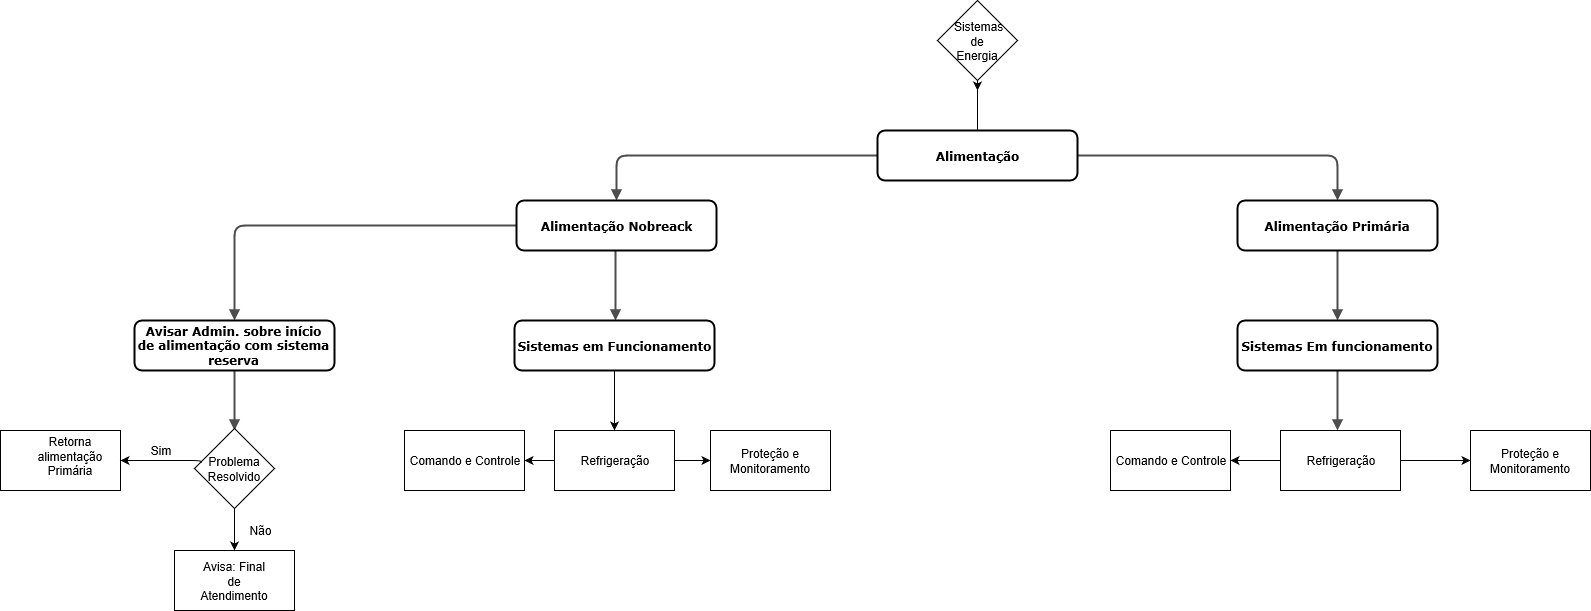
\includegraphics[scale= 0.3]{figuras/diagrama-funcional.jpg}
			\caption{Diagrama Funcional do Sistema.}
			\label{diagrama-funcional}
		\end{figure}	

		\begin{figure}[H]
			\centering
			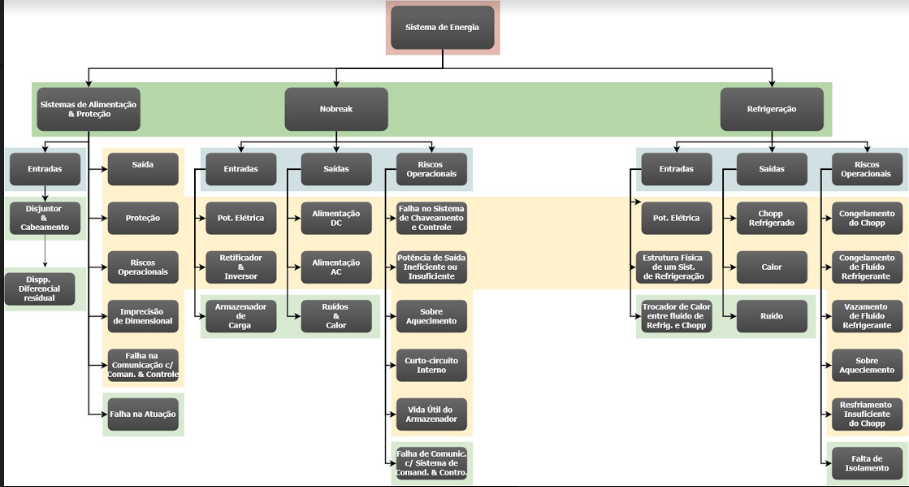
\includegraphics[scale= 0.55]{figuras/entradas-saidas.png}
			\caption{Entradas, saídas e riscos do sistema.}
			\label{entradas-saidas}
		\end{figure}	

		\subsubsection[Sistema de Refrigeração]{Sistema de Refrigeração}
			Para atender os requisitos estabelecidos no projeto no qual enquanto houver chopp na máquina esse permanecerá gelado para o consumo. Assim sendo, necessita-se implantar um ciclo de refrigeração. 
			
			O ciclo de refrigeração é um ciclo termodinâmico, no qual ocorre a retirada de calor de um ambiente. Esse ciclo é composto pelos seguintes itens: Evaporador, Compressor, Válvula de expansão e Condensador.
			
			O evaporador é um dispositivo que diminui a pressão do gás refrigerante, para que este diminua a temperatura e possa receber calor do ambiente a ser refrigerado. O compressor, por outro lado, irá comprimir o gás até a pressão do condensador, para que este condense e transfira o calor do gás para o ambiente, fazendo com que o gás fique no estado líquido e  retorne ao ciclo.

			\begin{figure}[H]
				\centering
				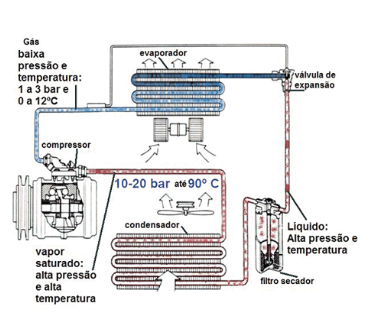
\includegraphics[scale= 0.7]{figuras/sistema-refrigerador.png}
				\caption{Ciclo Básico de Funcionamento do Sistema de Refrigeração.}
				\label{sistema-refrigerador}
			\end{figure}				

			Para o melhor entendimento do funcionamento do ciclo dito anteriormente observa-se a descrição dos processos termodinâmicos que ocorrem no mesmo abaixo: 

			\begin{figure}[H]
				\centering
				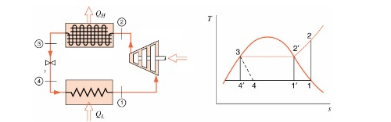
\includegraphics[scale= 0.7]{figuras/ciclo-termodinamico.png}
				\caption{Ciclo de Refrigeração e Ciclo termodinâmico.}
				\label{ciclo-termodinamico}
			\end{figure}				

			Nos processos 1-2 ocorre a compressão isentrópica do fluido refrigerante pelo compressor. Em seguida, nos processos 2-3 ocorre a transferência de calor a pressão constante ao reservatório ‘quente’ (condensador). Quando o fluido sai do processo 3 encaminha para a válvula isentrópica- processos 3-4. E por fim, segue para o processo 4-1 onde há transferência de calor a pressão constante ao ambiente que deseja refrigerar \cite{boles}.

			O evaporador no ciclo anteriormente citado consiste em um trocador de calor. Trocadores de calor sao dispositivos complicados. O aumento da transferência de calor em trocadores de calor e’ geralmente acompanhado com o aumento de pressão e, assim, uma maior potência de bombeamento. Sendo assim, qualquer ganho na transferência de calor deverá ser ser ponderada em relação ao custo da queda de pressão que o acompanha \cite{boles}.  

			Para o dimensionamento da taxa de transferência de calor do fluido refrigerante para o chopp usará a equação \ref{eq3}

				\begin{equation} 
					\label{eq3}
					Q = m \times {cp(T_{ent} - T_{sai})}
				\end{equation}

			A fórmula \ref{eq3} é usada antes mesmo de se ter informações a respeito sobre o trocador de calor que será utilizado.
			
			Para a implantação do sistema de refrigeração há dois tipos de trocadores de calor que podem ser adotados no projetos: Casco e tubo e Chirller de contra fluxo. Esses dois tipos de trocadores encontram-se ilustrados abaixo: 

			\begin{figure}[H]
				\centering
				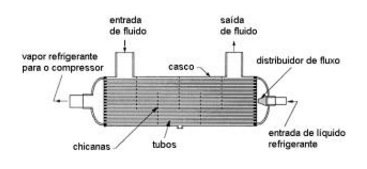
\includegraphics[scale= 0.7]{figuras/trocador-calor.png}
				\caption{Trocador de Calor do Tipo Casco e Tubo.}
				\label{trocador-calor}
			\end{figure}				


			\begin{figure}[H]
				\centering
				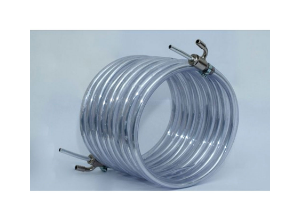
\includegraphics[scale= 0.7]{figuras/chirller.png}
				\caption{Chirller de Contra Fluxo.}
				\label{chirller}
			\end{figure}				
			
			O trocador de calor do tipo casco e tubo promove a flexibilidade quanto a disposição da area de transferencia de calor, assim sendo há diversas formas com que o trocador pode funcionar. Já o trocador do tipo Chirller de Contra Fluxo promove a ampliação de área de transferência de calor, facilidade de manutenção e de acesso para limpeza e consequentemente manutenção do produto. 
			
			Outra importante variável é a potência requerida do compressor. Este cálculo é feito observando a primeira lei da termodinâmica. Para um compressor temos:

			\begin{equation} 
				\label{eq4}
				W = m \times {(h_{2} - h_{1})}
			\end{equation}

			Onde:
				\begin{itemize}
					\item \textit{W} = Potência do compressor
					\item \textit{m} = fluxo mássico do gás
					\item \textit{h} = entalpia
				\end{itemize}

			Para encontrarmos os dados tabelados do fluido refrigerante de entrada e saída do compressor, sabe-se que a temperatura de entrada do fluido no compressor é de aproximadamente 25$^\circ$ e a pressão é 0,6bar ou 60KPa, e a temperatura de saída ultrapassa os 100$^\circ$ com pressão de aproximadamente 8bar ou 0,8MPa. O estado de entrada para ser observado em tabelas termodinâmicas é vapor saturado, e o de saída é vapor superaquecido. O dado encontrado de entalpia no estado 1 é 227,79 KJ/Kg e no estado 2 é 337,3 KJ/Kg. O fluxo mássico assumido é 0,005 Kg/s. Temos:

			\begin{equation}
				W = 547,55 W 
			\end{equation}

			Logo, a potência calculada do compressor é aproximadamente 600W, como um dos requisitos é que a máquina produza dois chopps diferentes, necessita-se de duas serpentinas, dobrando assim a potência do compressor, aproximadamente 1090 à 1200 W.
			A escolha do condensador é feita a partir do compressor, no mercado é vendido de acordo com a potência do compressor. 


		\subsection[NoBreak]{NoBreak}
			O Nobreak, será responsável por manter o funcionamento da máquina e seu sistema por determinado período (a ser estipulado) em que a alimentação principal esteja fora de funcionamento. Para tanto ele deve conter uma fonte individual, uma bateria, interligado a elemento conversor de corrente contínua e da tensão 12V da bateria  para corrente alternada, 220V e 60Hz para que seja capaz de suprir o sistema de refrigeração.

			Com relação à escolha da bateria, fonte que irá suprir o sistema Nobreak, esta deverá ser tal que ao serem contabilizados o consumo de cada elemento do projeto está deverá suprir à demanda desses por período a ser estipulado. Levando em consideração o maior absorvedor de potência do sistema, o sistema de refrigeração que consome cerca de 1.0 a 1.4 A( Dado obtido em catálogo da EMBRACO para compressores de 0.25HP), e tomando um aumento de consumo de 50\%\ para os demais sistemas e seus componentes, tem-se que o consumo médio seria de aproximadamente 2.0A.

			Logo, buscando na teoria verifica-se para que seja escolhida uma bateria, além de conhecer sobre a tensão e corrente que esta irá suprir, se deve conhecer suas curva de descarga (relação de decaimento da tensão disponível); capacidade de armazenamento de energia (mede a quantidade de carga que pode ser entregue em determinado período) e capacidade de descarga (capacidade de entrega de carga sem que haja danos a bateria) \cite{meggi}. Dos tipos de baterias disponíveis no mercado aquelas que são mais empregadas em aplicações que demandam elevadas correntes são as de chumbo ácido, devido a sua vida útil, de até 4 anos, e de seu custo benefício. 
			
			Abaixo pode ser verificado um circuito representativo de um sistema Nobreak meramente ilustrativo visto que a equipe optou para este projeto montar o sistema em questão, porém a retificação, controle, e inversão de sinal serão realizadas por dispositivo comercial, o inversor: 


			\begin{figure}[H]
				\centering
				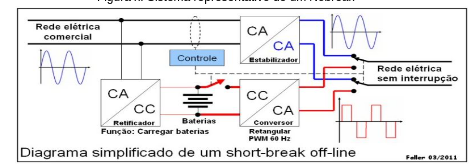
\includegraphics[scale= 0.7]{figuras/nobreak.png}
				\caption{Sistema representativo de um Nobreak.}
				\label{nobreak}
			\end{figure}		

		\subsection[Sistema de Alimentação]{Sistema de Alimentação}
			O sistema de alimentação principal será por meio de acesso à rede de distribuição por ponto de tomada, sendo esta de tensão nominal 220V e frequência de 60HZ. Há ainda a alimentação dos sistemas de comando e controle que será proveniente do mesmo acesso à rede, porém,  com inserção de uma fonte DC, visto que nestes sistemas é a mais usual devido a características específicas, tal como facilidade de controle.
			
			Serão utilizados cabeamentos multifilares de 4.5mm para cabos de fase e neutro e de 2.5mm para aterramento. Para os sistemas de comando e controle cabos de 0.5mm. De acordo com a norma ABNT NBR 5410: 2004.

		\subsection[Sistema de Proteção]{Sistema de Proteção}
			Interligado a ambos o sistemas de alimentação estará um quadro com dispositivos de proteção e segurança sendo composto por um disjuntor, um dispositivo diferencial residual e um botão de emergência a ser localizado em local mais acessível possível. O disjuntor é um dispositivo de proteção contra possíveis curtos circuitos. Já o dispositivo diferencial residual é para proteção contra choques e surtos elétricos no sistema, exigido por norma quando a instalação elétrica está em locais úmidos. 

			\begin{figure}[H]
				\centering
				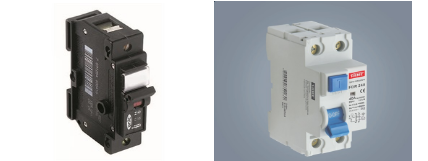
\includegraphics[scale= 0.7]{figuras/disjuntor.png}
				\caption{ A esquerda, disjuntor eletromecânico comercial; a direita Disjuntor Diferencial Residual.}
				\label{disjuntor}
			\end{figure}		